\section{Theorie}
Als erstes wird die Yagi-Uda-Antenne beschrieben. In einem zweiten Teil wird deren Strahlungsdiagramm betrachtet um die Abstrahlung zu verstehen. Dieses Kapitel dient der Erarbeitung der Theorie der Yagi-Uda-Antenne.

\subsection{Yagi-Uda-Antenne}\label{sec:Yagi}
Die Yagi-Uda-Antenne stammt aus Japan \cite{script}. 1926 erfanden Shintaro Uda und Hidetsugu Yagi die Antenne. Etwas später veröffentlichte Yagi den ersten englischen Artikel. Aus diesem Grund wir heute oft die Antenne nur noch mit dem Namen Yagi in Verbindung gebracht. Ein typisches Beispiel für die Verwendung einer Yagi-Antenne ist der Fernsehrundfunkempfang. Hierfür wird die Antenne für eine Frequenz von einigen \SI{100}{MHz} ausgelegt.

Zur Erhöhung der Richtwirkung können sowohl Reflektor- als auch Direktordipole an einen primär erregten Dipol angebracht werden. Oft wird eine ganze Reihe von Direktoren, bis zu 20 Stück, benutzt. Jedoch wird sich meist auf einen Reflektor beschränkt. Zur Minderung der unerwünschten Rückstrahlung wird zum Teil mit weiteren Stäben der Reflektor zu einer reflektierenden Wand ausgebaut.

In der Praxis werden als Reflektoren meist Halbwellendipole verwendet \cite{book}. Der aktive gespeiste Dipol wird etwa \SI{6}{\percent} kürzer ausgeführt. In der Direktorreihe wird jeder Nachfolger ungefähr \SI{1}{\percent} als sein Vorgänger ausgelegt. Die Elementabstände liegen um $0.3 \cdot \lambda $. Alle Strahler sind zentriert auf einem Trägerstab befestigt. Durch die Strahlungskopplung, welche mit zunehmendem Abstand schwächer wird, werden die passiven Dipole zum Mitschwingen angeregt. Die unterschiedlichen Längen der Elemente führen zu unterschiedlichen Phasenverschiebungen zwischen einfallender und abgestrahlter Welle. Diese Phasenverschiebung sowie der Abstand der Elemente werden so dimensioniert, dass es in Hauptstrahlungsrichtung zu einer konstruktiven Überlagerung der Teilwellen und damit zu einer starken Abstrahlung kommt. Je weiter die Elemente vom aktiven Dipol entfernt sind, desto weniger tragen sie zur Abstrahlung bei. Deshalb ist der erzielbare Gewinn einer Yagi-Antenne beschränkt. Wenn die Antennenlänge $L$ auf einen Wert im Bereich $ 0.5\leq L/\lambda_{0} \leq 7$ verdoppelt wird, steigt der Gewinn nur um \SI{2.2}{dB} und nicht um \SI{3}{dB}.

\begin{figure}[H]
	\centering
	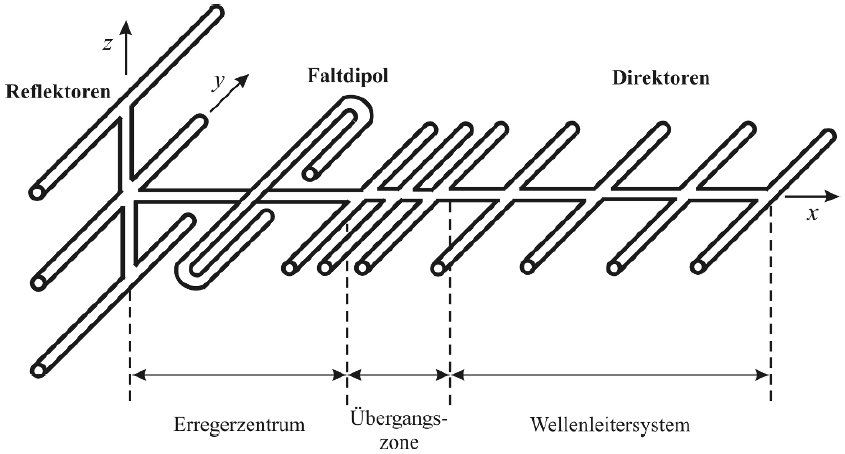
\includegraphics[width=0.8\linewidth]{yagi_antenne}
	\caption{Aufbau einer Yagi-Antenne mit einem aktiv gespeisten Faltdipol und parasitären Strahlerelementen \cite{book}.}\label{fig:yagi}
\end{figure}

Wie der Abbildung \ref{fig:yagi} entnommen werden kann, lässt sich die Yagi-Antenne in drei Wirkungszonen unterteilen. Diese sind das Erregerzentrum, die Übergangszone und das Wellenleitersystem.

\paragraph{Erregerzentrum}
Im Erregerzentrum wird die Bandbreite und der Eingangswiderstand der ganzen Antenne bestimmt. Durch die parasitären Elemente wird der Dipol stärker belastet. Deshalb wird der Strahlungswiderstand niederohmiger. Um dem entgegenzuwirken wird meistens ein Faltdipol verwendet, da er gegenüber einem "gestreckten" $\ \lambda/2 $-Dipol den Vorteil grösserer Breitbandigkeit und etwa viermal höheren Eingangswiderstand besitzt. Als Speiseleitung wird eine Flachbandleitung mit $ Z_{L} \approx 240\Omega $ an den Dipol angeschlossen. Der Reflektor gehört auch zum Erregerzentrum. Er kann mit zusätzlichen Stäben zu einer reflektierenden Wand erweitert werden.

\paragraph{Übergangszone}
Dieser Bereich besteht aus mehreren Direktoren. Sie dienen zur optimalen Anpassung der Strahlung des Erregerzenstrums an das folgende Wellenleitersystem.

\paragraph{Wellenleitersystem}
Mit diesem System wird die Strahlungscharakteristik der Antenne bestimmt. Es wird aus mehreren Direktoren gebildet.

\subsection{Strahlungsdiagramm}\label{sec:Strahlungsdiagramm}

Das Strahlungsdiagramm wird benutzt um  graphisch die Richtcharakteristik einer Antenne darzustellen. Das Diagramm gibt Informationen über die Feldstärkenverteilung von der Antenne in grosser Distanz. In der Abbildung \ref{fig:richtdiagram} ist das 3D-Strahlungsdiagramm einer Yagi-Antenne dargestellt. Die Hauptstahlrichtung der Antenne breitet sich zur Richtung des Direktors aus.

\begin{figure}[H]
	\centering
	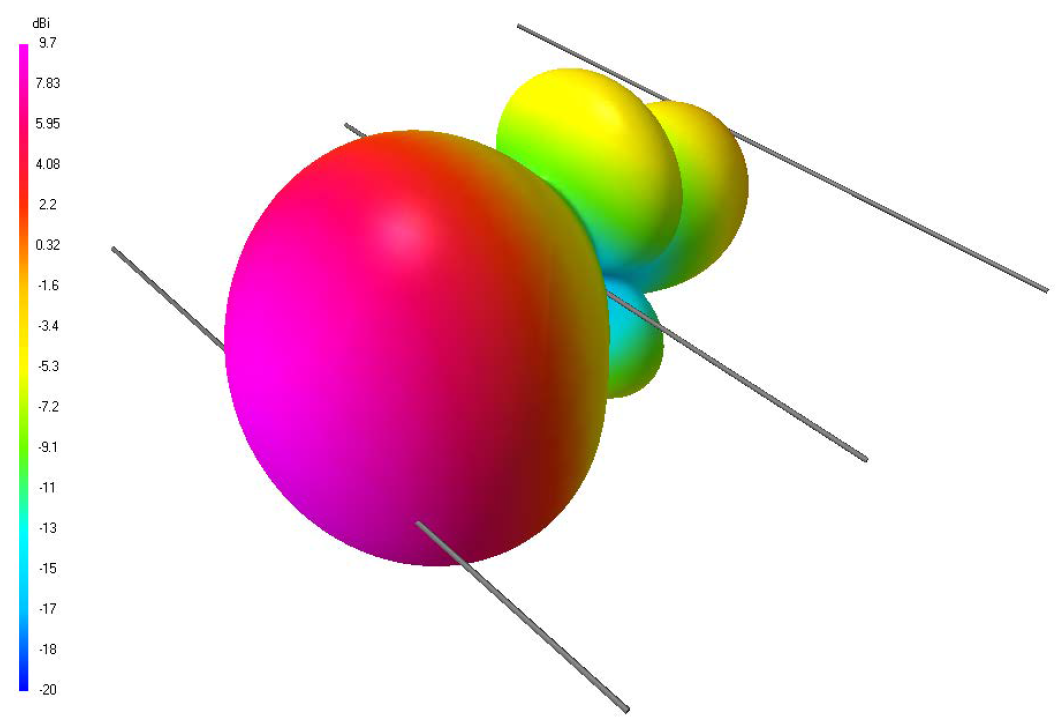
\includegraphics[width=0.8\linewidth]{yagi_richtdiagram}
	\caption{3D-Strahlungsdiagramm einer Yagi-Antenne mit einem Direktor \cite{script}.}\label{fig:richtdiagram}
\end{figure}
